\documentclass[color, ddc]{tudscrreprt}
%\usepackage[T1]{fontenc}
% Achtung: LuaLaTeX!!
\usepackage[utf8]{luainputenc}
\usepackage[ngerman]{babel} 
\usepackage{underscore}
\usepackage[colorlinks=false,hidelinks]{hyperref}

\let\myBib\thebibliography
\let\endmyBib\endthebibliography
\renewcommand\thebibliography[1]{\ifx\relax#1\relax\else\myBib{#1}\fi}

\usepackage{graphicx}
\usepackage{grffile}
\shorthandoff{"}	

\faculty{Fakultät Elektro- und Informationstechnik}
\chair{Institut für Automatisierungstechnik}
\begin{document}
    \title{Dokumentation Praktikum Mensch-Maschine-Systemtechnik}
    \subtitle{Entwurf einer Visualisierung für das
semantische Revisionsverwaltungssystem R43ples}
    \author{Gruppe 2.3:
    Lukas Buntkiel, 
    Alexander Lehmann, 
    Miao Zhang, 
    Sven Schönfeld,
    Falk-Jonatan Strube}
    \maketitle

\tableofcontents

\chapter{Einleitung}

\section{Einordnung}

Hauptbestandteil der Aufgabenstellung ist das Entwerfen einer interaktiven Darstellung der Revisions-Struktur des Versionsverwaltungssystems (Version Control System, VCS) R43ples.

R43ples kann zur Versionsverwaltung von Named Graphs genutzt werden, dem Schlüs\-sel-Be\-stand\-teil des Semantic Web \cite{pascal:semanic-web}. Es verwendet dabei zur Verwaltung der Revisionen wiederum Named Graphs, in denen auch sämtliche, zur Darstellung der Struktur notwendigen, Informationen in Form von Linked Data enthalten sind \cite{graube:r43ples}. R43ples verwendet dabei ein ähnliches Konzept wie klassische Versionsverwaltungssysteme (wie z.B. git \cite{url:git-scm}) indem es Verzweigungen von Revisionen in Form von Branches sowie das Kennzeichnen spezieller Revisionen mit Tags unterstützt \cite{graube:r43ples}.

Der Hauptunterschied zu klassischen VCS liegt also weniger im Konzept der Versionsverwaltung selbst, als in der Anwendung dieses Konzeptes auf einen neuen Typ von Ressource (Named-Graphs). Es kann daher angenommen werden, dass durch andere VCS bereits Lösungen für die graphische Darstellung von Revisionen vorhanden sind, die im Verlauf dieser Arbeit analysiert werden können, um günstige Merkmale herauszuarbeiten.

\section{Theoriebildung}

Die durch den Lehrstuhl gegebene Aufgabenstellung lautet wie folgt:

\begin{quotation}
Ziel dieser Aufgabe ist es, eine gebrauchstaugliche Visualisierung für das semantische Revisionsverwaltungssystem R43ples) zu implementieren, die Revisionsgraphen mit Branches, Merges und Tags darstellen kann. Das Werkzeug soll sich nahtlos in die HTML-Oberfläche des Gesamtsystems einfügen und dem Nutzer Überblicksinformationen über den Revisionsverlauf und Detailinformationen zu den einzelnen Revisionen geben.
\end{quotation}

Dem entsprechend wurden bei der Theoriebildung folgende Kernanforderungen an das Projekt herausgearbeitet.

\paragraph{Schnittstelle zu bestehender Software}

Zuerst muss eine Schnittstelle zur bestehenden Software hergestellt werden. Das wäre möglich, indem man beispielsweise die turtle Datensätze ausliest die der laufende Server ausgibt. Dadurch hätte man ein separates System das unabhängig vom Revisions-Server turtle Datensätze auslesen und darstellen könnte.

Eine andere Möglichkeit stellt die direkte Integration in das R43ples-Projekt auf github dar, in der Visualisierung direkt im System integriert wäre. Diese Herangehensweise hätte den Vorteil, dass man nicht erst eine turtle Datei parsen müsste, sondern direkt auf die Datensysteme des Servers zugreifen könnte. Durch einen fork des repositorys könnte man an einer Lösung der Aufgabe arbeiten und hätte bei einer guten Lösung einen einfachen Weg die Ergebnisse schnell im Hauptprojekt zu nutzen.

\paragraph{Graphische Darstellung realisieren}

Nachdem die Daten für das System über die Schnittstelle beschafft wurden, ist eine Hauptaufgabe diese als graphische Darstellung zu realisieren.

Eine erste Realisierung liegt bereits als einfache Implementierung mit Viz.js vor. 
Diese ist allerdings als nicht besonders gut und lediglich als Platzhalter zu bewerten.

Der Graph wird anscheinend nach keinen gestalterischen Grundsätzen generiert. Bis auf die chronologische Auflistung der Revisionen von oben nach unten und die Pfeile als optische Hilfestellung wird keine weitere Hilfestellung geboten, die die Erfassung des Graphen erleichtern würde.

Des weiteren ist die Auswahl der Informationen die von den Revisionen angezeigt werden nicht optimal. Sie bietet dem Nutzer nur zwei Informationen, wobei eine davon für den Nutzer uninteressant ist. Es fehlen aber andere wie beispielsweise der Autor oder das Datum.

\begin{figure}[ht!]
\centering
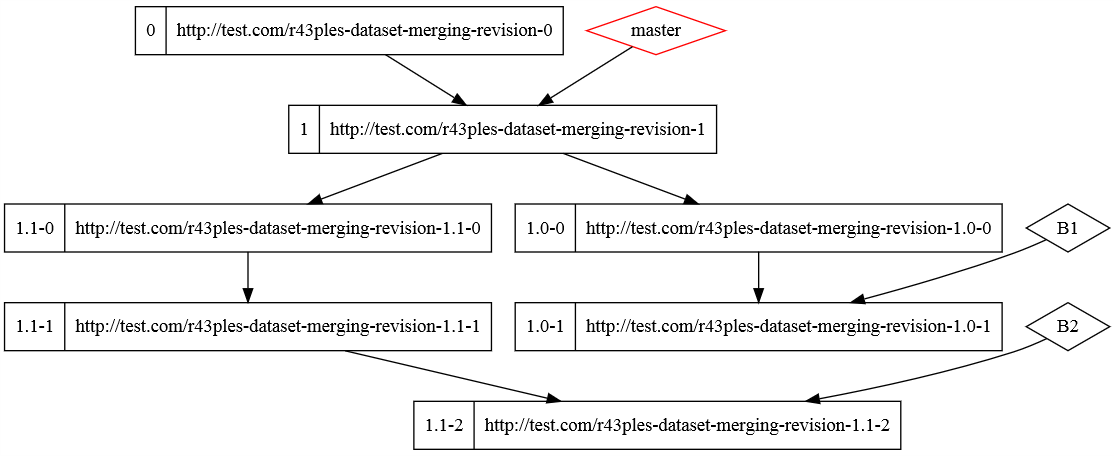
\includegraphics[width=\textwidth]{Skizzen/vizjs.png}
\caption{Vorgegebene Implementierung mit Viz.js}
\end{figure}

\paragraph{Überblicks- und Detailsicht}

Wenn man die Idee der vorhandenen Implementierung beibehalten möchte, die die Informationen der Revisionen direkt in den Knoten des Graphen darstellt muss man sich überlegen, wie man bei großen Revisionsbäumen eine übersichtliche Darstellung erreicht.

Um einen guten Kompromiss aus Informationsfülle und Übersichtlichkeit zu finden würde sich also vor allem bei vielen Daten ein Trennung des Graphen in eine Überblicks- und eine Detailansicht anbieten. So könnte man in einem Überblicksgraphen die wichtigsten Informationen anzeigen und durch das Navigieren auf eine spezielle Revision eine Detailansicht erreichen, die sämtliche relevanten Informationen darstellt.

\subsection*{Wie visualisiert man ein semantisches Versionsverwaltungssystem?}

%Die Frage die sich also stellt ist, wie man ein semantisches Versionsverwaltungssystem am besten darstellt.

Wie bereits in der Einordnung erwähnt, kann als Konzept ein ähnliches verwendet werden wie ein klassischen Versionsverwaltungssystemen. Folgende Richtlinien wurden als Gestaltungsgrundsatz festgelegt:
\begin{itemize}
\item Übersichtlichkeit -- alle wichtigen Informationen sollen mit einem Blick gesehen werden
\item Verständlichkeit -- alle gesehenen Informationen sollen möglichst schnell im Zusammenhang verstanden werden
\item Angemessener Informationsgehalt -- Je nach Ansicht sollen angemessen viele Informationen dargestellt werden nach dem Motto: „so wenig wie möglich, so viel wie nötig“
\end{itemize}

\section{Literatur}

Nachdem in der Einordnung die grundlegende Literatur für das Thema dargelegt wurde (\cite{pascal:semanic-web}, \cite{graube:r43ples}, \cite{url:git}), finden sich auch noch mehr Informationen in verschiedensten wissenschaftlichen Publikationen:

Der Artikel „Special Graph Representations And Visualization Of Semantic Networks“ \cite{borisenko:graph-representation} steigt genau bei der Fragestellung nach der Visualisierung von semantischen Netzwerken ein und bietet einen grundlegenden Überklick für die Herangehensweise.

Die Masterarbeit „Ein empirischer Vergleich von semistrukturierter und unstrukturierter Konfliktbehandlung in Versionsverwaltungssystemen“ \cite{brandl:versionsverwaltung} gibt dabei einen tieferen Einblick zu einem Aspekt der Versionsverwaltung, ist bei der Visualisierung aber nur bedingt hilfreich.

In „Approaches to Visualising Linked Data: A Survey“ \cite{dadzie:linked-data} wird zwar die Visualisierung von Linked Data vorgestellt, allerdings weniger im Bereich der Graphenbildung. Dadurch ist der Artikel für dieses Projekt in dem die Daten durch einen Graphen geordnet darstellen wollen weniger bedeutsam.

Ganz ähnlich bietet „A General Introduction To Graph Visualization Techniques“ \cite{tarawneh:graph-visualization} einen Überblick über die Visualisierungs-Optionen, wobei hier vermehrt Lösungen durch Graphen vorgestellt werden, was den Artikel etwas interessanter für das Projekt macht.

Dann bietet sich nach der Theoriebildung an sich Literatur zu den gefundenen Problem- und Fragestellungen zu suchen.

Der Artikel „Eye tracking for visualization evaluation: Reading values on linear versus radial graphs“ \cite{goldberg:visualization-evaluation} führt auf, was die Unterschiede sind, ob man Graphen linear oder radial darstellt. Dabei wird der Schluss präsentiert, dass linear dargestellte Graphen deutlich einfacher auf den ersten Blick zu erfassen sind, weswegen in dem Projekt eine solche Darstellung verwendet werden soll.

Die im Internet zu findende Seite „A successful Git branching model“ \cite{driessen:branching-model} zeigt schon auf eine gute Weise, wie man ein Versionsprotokoll darstellen kann und worauf zu achten ist.

Die DIN „Software-Ergonomie für Multimedia-Benutzungsschnittstellen“ DIN EN ISO 14915 \cite{DIN:EN-ISO-14915-1} \cite{DIN:EN-ISO-14915-2} \cite{DIN:EN-ISO-14915-3} gibt entscheidende Richtlinien für die Gestaltung des Projektes im Rahmen einer Benutzerschnittstelle, was vor allem dann von Bedeutung ist, falls die verschiedenen Ansichten in ihren Zoom-Stufen umgesetzt werden soll.
    
\chapter{Analyse und Entwurf}

\section{Analyse}

\paragraph{Darstellungen anderer Subversion Systeme}
\begin{figure}[ht!]
\centering
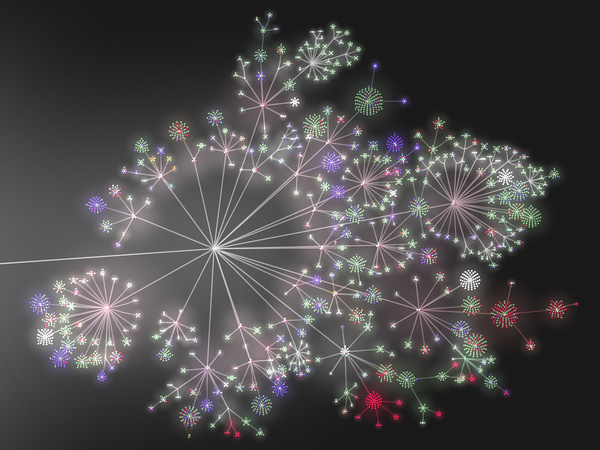
\includegraphics[width=0.5\textwidth]{Skizzen/gource.jpg}
\caption{gource Visualisierung}
\end{figure}

\begin{figure}[ht!]
\centering
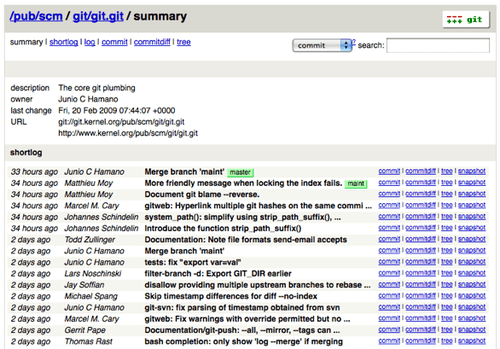
\includegraphics[width=0.5\textwidth]{Skizzen/gitweb.png}
\caption{gitweb Visualisierung}
\end{figure}

\begin{figure}[ht!]
\centering
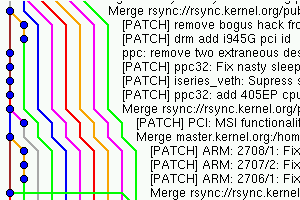
\includegraphics[width=0.5\textwidth]{Skizzen/gitready-gitk.png}
\caption{gitready Visualisierung}
\end{figure}
\begin{itemize}
\item SVN \cite{url:svn-gource}
\item GIT \cite{url:git}
\item GIT \cite{url:gitready}
\end{itemize}

\section{Entwurf}

\newpage
\begin{figure}[ht!]
\centering
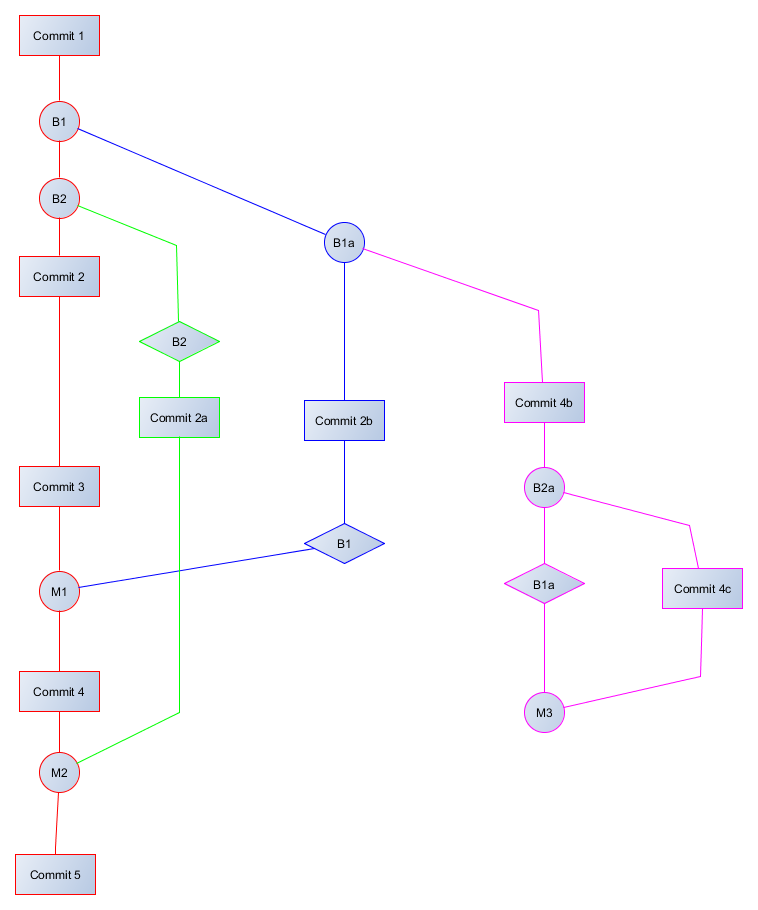
\includegraphics[width=\textwidth]{Skizzen/2014-12-12 VisualisierungsSkizze.png}
\caption{Erste Skizze}
\end{figure}

\newpage
\begin{figure}[ht!]
\centering
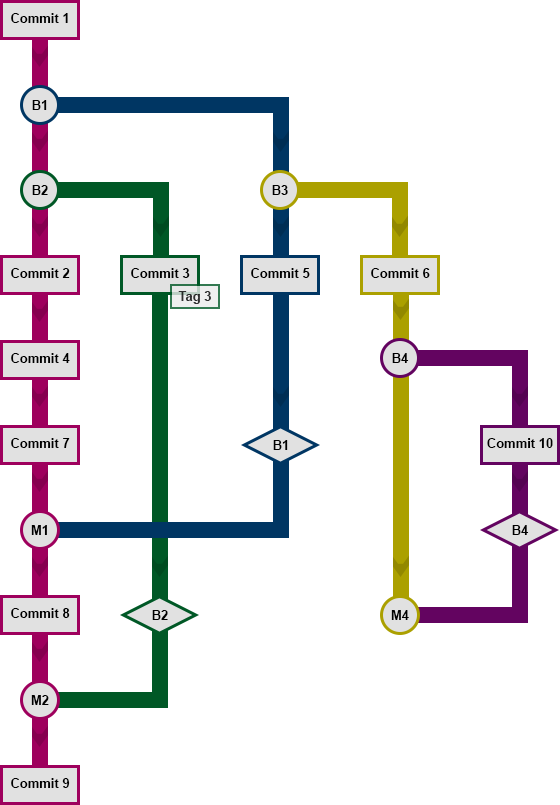
\includegraphics[width=\textwidth]{Skizzen/2015-01 VisualisierungsSkizze-rev.png}
\caption{Überarbeitete Skizze}
\end{figure}

\chapter{Pflichtenheft}

Die Erstellung des Pflichtenhefts erfolgt entsprechend der Empfehlungen des IEEE Guide for Software Requirements Specifications (SRS) \cite{ieee1998ieee}. Die dort empfohlene Struktur wird in deutscher Übersetzung nach Balzert \cite{balzert2009lehrbuch} übernommen.

\section{Produktfunktionen}
\subsection{Muss}
\begin{itemize}
\item Daten (bspw. aus turtle-Datensatz) auslesen (zum weiterverarbeiten)
\item Daten werden graphisch abgebildet
\end{itemize}

\subsection{Kann}
\begin{itemize}
\item Daten werden in in unterschiedlichen Darstellungsebenen dargestellt (Gesamt- und Detailübersicht)
\item Einzelansicht für die Details von Revisions
\item Daten werden tabellarisch-strukturiert abgebildet
\end{itemize}

\subsection{Soll}
\begin{itemize}
\item Zweckmäßige Übergangsanimationen zwischen Darstellungsansichten
\end{itemize}

\section{Qualitätsanforderungen}
\begin{itemize}
\item Daten werden unverfälscht abgebildet
\item Durch Informationsreduzierung (auf das nötigste) wird ein höhere Übersichtlichkeit erreicht (Minimierung der Darstellung von merges und revisions durch Unterteilung in Detailansichten)
\end{itemize}

\section{Einschränkungen und Randbedingungen}
\begin{itemize}
\item Läuft auf neuerem Firefox und Chrome
\end{itemize}

\section{Annahmen und Abhängigkeiten}
\begin{itemize}
\item Nutzer ist mit r43ples und dem semantic web vertraut
\end{itemize}

\chapter{Gestaltungsentwurf}

\begin{itemize}
\item Framework zu svg-Generierung: Apache Batik
\begin{itemize}
\item implementiert die Java Graphics2D API → Code zum Zeichnen kann wiederverwendet werden, z.B. auf einem AWT Canvas
\end{itemize}
\item Neue Datenstruktur „StructuredTree“ bildet den Commitgraph ab und vereinfacht das Arbeiten mit den Commits
\begin{itemize}
\item beinhaltet doppelt verknüpften Graphen der Commits, Liste der Branches und Liste der Tags, beides jeweils mit Referenzen auf die Commits
\item kapselt die Logik zum Generieren der Datenstruktur aus dem SPARQL Result
\end{itemize}
\item Trennung von Commit-Graph und Zusatzinformationen durch Regel: Ein Commit pro Zeile
\begin{itemize}
\item → bessere Übersichtlichkeit für den Anwender, da die Beschriftungen nicht die Außmaße des Graphen vergrößern → Graph bleibt kompakt, geringe Augenbewegungen nötig um den Graphen vollständig zu erfassen.
\item Reihenfolge der Commits sofort erkennbar, da pro Zeile nur ein Commit
\item Um von Commit-„Punkt“ im Graphen zur Beschriftung zu gelangen nur eine geradlinige horizontale Augenbewegung nötig → trotz Trennung hohe Lesegeschwindigkeit (siehe Literatur: „Information Visualisation“)
\end{itemize}
\item Commit-Graph verläuft in Spalten, pro Spalte ein Branch → gute Übersichtlichkeit
\begin{itemize}
\item verschiedene Spalten außerdem verschieden eingefärbt → ebenfalls Erhöhung der Übersichtlichkeit
\item Farbwahl sollte der Ermüdung des Auges verbeugen
\end{itemize}
\item Zeitpunkt des Commits wird nur tagesgenau wiedergegeben + Ausgabe des Datums nur wenn Änderung zu vorhergehendem Commit → Herabsetzen des Informationsgehaltes und Vermeiden von Redundanzen damit der Anwender die Daten schneller überblicken kann
\end{itemize}

%\chapter{Abgabe}

\bibliographystyle{unsrt}
\bibliography{Literatur}

\end{document}